\documentclass%
% Obligatory: Adjust BCOR depending on your type of binding for proper
% binding correction! See https://ftp.fau.de/ctan/macros/latex/contrib/koma-script/doc/scrguien.pdf#section.2.6 .
[ BCOR=1cm
% We strongly advise you to use a two-sided layout.
, twoside
]{dpmthsis}


\usepackage[german]{babel}
\usepackage{float}

\usepackage{subcaption}

\usepackage{rotating}
\usepackage[dvipsnames]{xcolor}


\usepackage[backend=biber,style=alphabetic]{biblatex}
\addbibresource{References.bib}


\begin{document}


\frontmatter
\pagestyle{empty}


\includepdf{out/CoverDE.pdf}

\cleardoublepage

\section*{Zusammenfassung}


TODO


\cleardoublepage


\tableofcontents
\listoffigures


\mainmatter
\pagestyle{headings}


\chapter{Motivation und Aufbau}
\label{Motivation und Aufbau}

Das klassische Genetic Programming (GP) wird heutzutage für die Problemlösung in den unterschiedlichsten Domänen erforscht.
Beispiele hierfür sind die Erstellung einer mathematischen Gleichung für einen industriellen Prozess \cite{sette_genetic_2001}, die Strukturanalyse von FGMs (funktionell gradierten Materialien) \cite{demirbas_stress_2022} und der Verarbeitung von natürlicher Sprache \cite{araujo_genetic_2020}.

Cartesian Genetic Programming (CGP) ist eine Methode des GPs, in der Lösungen für Probleme als Graphen dargestellt werden \cite{miller_cartesian_2020}. 
Im Standard-CGP werde laut Miller der Rekombinationsschritt normalerweise nicht ausgeführt und in den meisten Arbeiten werde dieser Schritt gänzlich ignoriert. 
Er bezieht dieses Verhalten auf Forschungsergebnisse aus dem Jahr 1999, die nach Miller aufzeigen, dass der Rekombinationsschritt kaum einen Effekt auf die Effizienz von CGP hat. \cite{miller_cartesian_2020} 
In mehreren weiteren Papern werden andere Rekombinationsalgorithmen mit dem Ziel vorgestellt, dass der Rekombinationsschritt neben der Mutation sinnvoll in CGP eingebaut werden kann. 
Dieser weitere Operator könnte die Effizienz von CGP-Modellen im Training steigern und somit komplexere Ausgangsprobleme lösbar machen.
Innerhalb dieser Paper wird als Prämisse angenommen, dass wie von Miller geschildert in Standard-CGP keine Rekombination verwendet wird. \cite{clegg_new_2007,kalkreuth_comprehensive_2020, torabi_using_2022}\\
Da die Aussage, dass in Sandard-CGP der Rekombinationsschritt nicht zielführend sei, auf den Papern von Miller aus dem Jahr 1999 und 2011 basiert, kommt die Frage auf, ob dies immer noch zutrifft.
Die erste Forschungsfrage, die in dieser Arbeit beantwortet werden soll, ist demnach: \glqq Kann nach heutigem Forschungsstand Rekombination die Effizienz von Standard-CGP steigern?\grqq

Da der Erfolg der Rekombination ebenfalls von der Rekombinationsrate abhängt, ist es sinnvoll diese näher zu betrachten. 
Clegg et al. und Torabi et al. beschreiben in ihren Papern unterschiedliche Herangehensweisen an die Rekombinationsrate \cite{clegg_new_2007, torabi_using_2022}:\\
Clegg et al. führen eine variable Rekombinationsrate in ihrem Paper ein.
Dabei wird eine hohe Rekombinationsrate linear verringert, sodass in den letzten Lernschritten keine Rekombination mehr ausgeführt wird. \cite{clegg_new_2007}\\
Torabi et al. fügen für ihre Rekombination ein Offset zu Beginn des CGP ein. 
Dieser Offset wird durch einen Hyperparameter bestimmt und gibt an, wie viele Iterationen die Rekombination ausbleibt. \cite{torabi_using_2022}\\
Diese beiden Ansätze sollen mit einem selbst entwickelten Ansatz verglichen werden.
Die neu vorgestellte Rekombinationsrate bezieht sich auf die One-Fifth-Rule zur Berechnung der Mutationsrate.
Auf Basis dessen ergibt sich die zweite Forschungsfrage: \glqq Hat die Art und Weise der Rekombinationsratenberechnung eine Auswirkung auf die Effektivität des CGPs?\grqq

Die beiden Forschungsfragen sollen anhand unterschiedlicher Experimente beantwortet werden.
In Abschnitt \ref{Grundlagen} werden die theoretischen Grundlagen erläutert, die für das Verständnis des Experimentaufbaus und der Ergebnisse benötigt werden.
Im Anschluss werden in Abschnitt \ref{praktischer Teil} die jeweiligen Experimente, sowie die Evaluationsstrategien der Ergebnisse beschrieben.
Darauf folgend werden in Abschnitt \ref{Ergebnisse} die Ergebnisse der Experimente vorgestellt und ausgewertet.
Abschließend wird in Abschnitt \ref{Fazit} ein Fazit aus den Ergebnissen zusammengefasst, sowie ein Ausblick auf weitere mögliche Forschungsfragen gegeben.

\chapter{Grundlagen}
\label{Grundlagen}

Für den praktischen Teil dieser Arbeit werden mit Hilfe von CGP unterschiedliche Testprobleme gelöst. 
Für das Verständnis dieses Teil werden einige Grundkenntnisse vorausgesetzt, welche in diesem Abschnitt näher betrachtet werden.\newline
CGP ist eine Art von GP, welches verwendet wird, um unterschiedliche Probleme zu lösen.
Dabei wird der Maschine allerdings nicht beigebracht, wie diese Probleme zu lösen sind.
Stattdessen lernt sie eigenständig über mehrere Iterationen hinweg das Ausgangsproblem zu lösen.
Dies geschieht angelehnt an die Darwin’sche Theorie der biologischen Evolution. \cite{milad_taleby_ahvanooey_survey_2019} \newline
Um den grundlegenden Aufbau von CGP zu erläutern, wird folgende Abbildung eingeführt:

\begin{figure}[H]
    \centering
    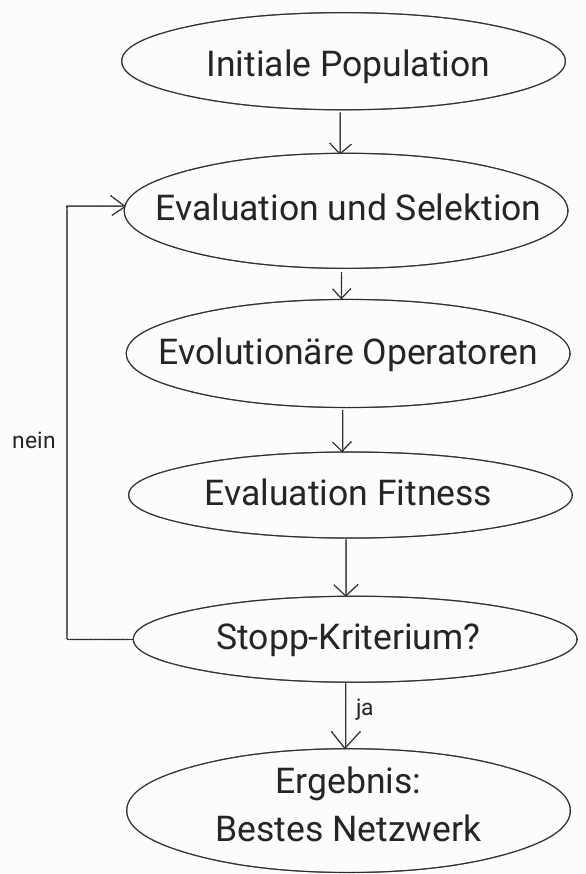
\includegraphics[scale = 0.52]{Bilder/AufbauCGPVorgehenNachbildung.png}
    \caption{Aufbau CGP, angelehnt an \cite{torabi_using_2022}}
    \label{fig:aufbauCGP}
\end{figure}

Die Abbildung zeigt den grundlegenden Ablauf innerhalb von CGP.
Dabei lernt das System über mehrere Iterationen hinweg die beste Lösung eines Problems.
Die folgenden Unterkapitel beziehen sich jeweils auf einen Knoten des Graphen und erläutern diesen genauer.


\section{Initiale Population}
\label{sec:initialePopulation}
Die Initialisierung der Population bezieht sich auf die Paper \cite{miller_cartesian_2020}, \cite{torabi_using_2022} und \cite{milad_taleby_ahvanooey_survey_2019}.
Außerdem werden Erkenntnisse aus dem Quellcode von Cui verwendet \cite{cuihen_cuihencgp_with_crossover_strategies_2024}.\\

Die Population von CGP ist eine Menge von Chromosomen oder auch Individuen genannt.
Chromosome sind individuelle Möglichkeiten ein komplexes Ausgangsproblem zu lösen.
Jedes Chromosom ist in CGP ein gerichteter, azyklischer Graph, bestehend aus Eingang-Knoten, Rechen-Knoten und Ausgang-Knoten.
Dabei gibt es zwei Darstellungsmöglichkeiten für ein Chromosom: den Genotyp und den daraus resultierenden Phänotyp.
Anhand der folgenden Abbildungen kann beispielhaft näher erläutert werden, wie die Chromosome in CGP aussehen und funktionieren. Dieses Beispiel wird in \cite{torabi_using_2022} eingeführt.

\begin{figure}[H]
    \centering
    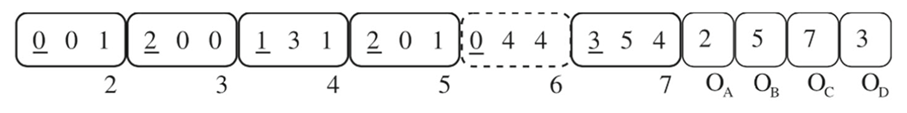
\includegraphics[scale = 0.6]{Bilder/TorabiBeispielGenotyp.png}
    \caption{Beispiel Genotyp, \cite{torabi_using_2022}}
    \label{fig:genotyp}
    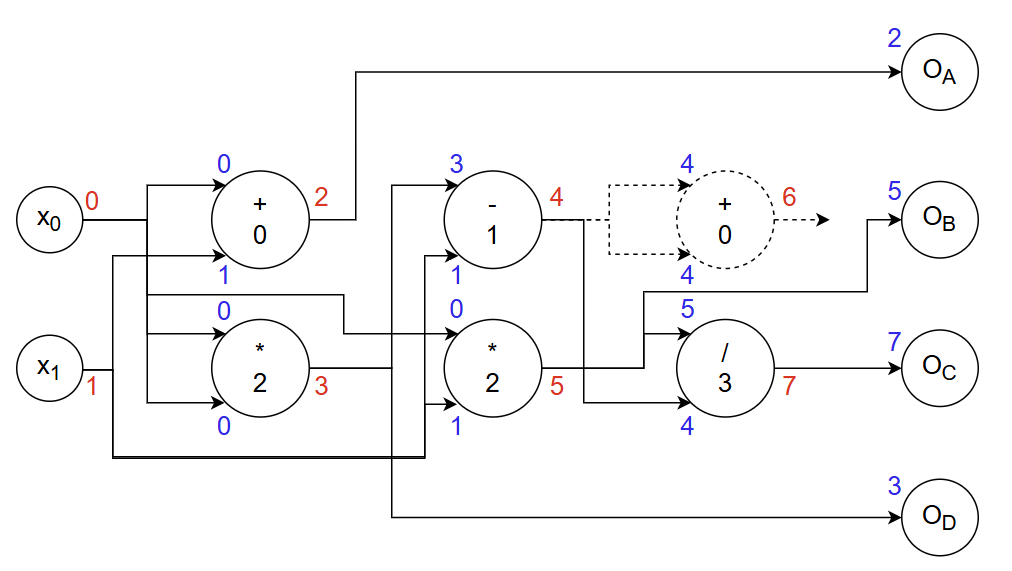
\includegraphics[scale = 0.5]{Bilder/BeispielChromosom.png}
    \caption{Beispiel Phänotyp, angelehnt an \cite{torabi_using_2022}}
    \label{fig:phänotyp}
\end{figure}

Abbildung \ref{fig:genotyp} zeigt einen Genotyp und Abbildung \ref{fig:phänotyp} den daraus resultierenden Phänotyp.
Anhand des Phänotyps lässt sich die klassische Struktur von CGP erkennen:
Es handelt sich um einen gerichteten, azyklischen Graphen mit Ein- und Ausgängen.
Bei den Eingängen (hier: $x_0$ und $x_1$) handelt es sich um die Systemeingänge, aus denen Ausgänge (hier: $O_A$ – $O_D$) abgeleitet werden sollen.
Zwischen den Ein- und Ausgangsknoten liegen die Rechenknoten.
Diese werden verwendet, um verschiedene Rechenoperationen an den Eingangsknoten auszuführen, bis schließlich die Inhalte der Ausgangsknoten als Ergebnis resultieren.
Die Rechenoperationen, die von den Rechenknoten ausgeführt werden, werden je nach Anwendungsfall definiert und codiert.
In diesem Beispiel ergibt sich folgende Kodierung:

\begin{table}[h]
    \centering
    \begin{tabular}{c|c}
       \textbf{Rechenoperation} & \textbf{Kodierung} \\ \hline
        + & 0 \\ \hline
        - & 1 \\ \hline
        * & 2 \\ \hline
        / & 3
    \end{tabular}
\end{table}

Diese Kodierungen werden im Phänotyp innerhalb der Knoten angegeben und stellen die erste (unterstrichene) Zahl innerhalb der Genotyp-Arrays dar.
Ein Genotyp-Array wird in Abbildung \ref{fig:genotyp} umrandet dargestellt und steht jeweils für einen Knoten.
Unterhalb dieser Array-Blöcke wird jeweils der Index des zugehörigen Knotens angegeben.
Im Phänotyp wird dieser Index am Ausgang des jeweiligen Knotens (rot) angezeigt.\newline
Des Weiteren werden im Genotyp die Eingangskanten für jeden Knoten angegeben. 
In diesem Beispiel hat jeder Rechenknoten zwei Eingänge und jeder Ausgangsknoten hat jeweils nur einen Eingang, in dem das Ergebnis eines Rechenknoten weitergeleitet und ausgegeben wird.
Die Knoteneingänge sind in Abbildung \ref{fig:phänotyp} blau markiert.
Hier werden die Indices derjenigen Knoten angegeben, deren Ausgangswerte verwendet werden.
Diese spiegeln sich ebenfalls im Genotyp wider: hier werden die Knoteneingänge innerhalb der Array-Blöcke als nicht-unterstrichene Indices angegeben.
Damit ergibt sich eine vollständige Beschreibung eines Knotens: einem Index werden Eingänge und gegebenenfalls eine Rechenoperation zugeschrieben.\newline
Durch dieses Beispiel wird ebenfalls ersichtlich, was die Eingangsknoten eines Chromosoms ausmacht:
Sie geben die Systemeingänge wieder, ohne diese auf irgendeine Weise zu verarbeiten.
Aus diesem Grund müssen die Eingangsknoten nicht im Genotyp aufgezeigt werden, sie vollständig zu beschreiben: sie weisen weder Eingänge noch Rechenoperationen auf, die beschrieben werden müssten.\newline
Als letzter Punkt fällt innerhalb des Beispiels auf, dass ein Knoten und dessen Kanten mit gestrichelten Linien dargestellt sind.
Dies ist ein sogenannter inaktiver Knoten und wird für die Berechnung des Endergebnisses nicht gebraucht.
Ob ein Knoten verwendet wird oder nicht, hängt davon ab, ob ein nachfolgender Knoten auf dessen Ausgang zugreift.
Um aktive Knoten von inaktiven Knoten zu unterscheiden, werden demnach zuerst die Ausgangsknoten betrachtet, die offensichtlich für die Auswertung der Ausgabe verwendet werden.
Anschließend werden iterativ die Eingangskanten der Rechenknoten zurückverfolgt, bis man schließlich bei den Eingangsknoten des Graphen ankommt.
Alle Knoten, die bis dahin besucht wurden, werden aktive Knoten genannt und sind für die Berechnung des Endergebnisses eines Chromosoms relevant. \newline
Schließlich soll anhand der eingeführten Abbildung ein Beispiel berechnet werden:\newline
Anzunehmen sind die Eingänge $x_0$ = 10 und $x_1$ = 20.
Demnach sind die Ausgänge der beiden Eingangsknoten mit den Indices 0 und 1 gleich den Werten 10 und 20.
Der erste Rechenknoten (Index = 2) verwendet als Eingänge die beiden Eingangsknoten (Indices = 0 und 1) und besitzt die Rechenfunktion +.
Demnach ist das Ergebnis des Rechenknotens (10 + 20 =) 30.
Führt man dieses Vorgehen für die restlichen Rechenknoten aus, ergeben sich folgende Ergebnisse:

\begin{table}[h]
    \centering
    \begin{tabular}{c|c|c|c|c}
       \textbf{Knoten} & \textbf{Eingänge} & \textbf{Werte Eingänge} & \textbf{Rechenoperation} & \textbf{Ausgangswert} \\ \hline
        2 & 0; 1 & 10; 20 & 10 + 20 & 30 \\ \hline
        3 & 0; 0 & 10; 10 & 10 * 10 & 100 \\ \hline
        4 & 3; 1 & 100; 20 & 100 - 20 & 80 \\ \hline
        5 & 0; 1 & 10; 20 & 10 * 20 & 200 \\ \hline
        7 & 5; 4 & 200; 80 & 200 / 80 & 2,5
    \end{tabular}
\end{table}

Die Ausgangsknoten geben die jeweiligen Ergebnisse der Eingangs- oder Rechenknoten zurück.
In diesem Beispiel werden durch das Chromosom die folgenden Ausgänge aus den beiden Eingängen (10; 20) berechnet:

\begin{table}[h]
    \centering
    \begin{tabular}{c|c|c}
       \textbf{Ausgangsknoten} & \textbf{Index Eingang} & \textbf{Wert des Ausgangsknotens} \\ \hline
        $O_A$ & 2 & 30 \\ \hline
        $O_B$ & 5 & 200 \\ \hline
        $O_C$ & 7 & 2,5 \\ \hline
        $O_D$ & 3 & 100
    \end{tabular}
\end{table}

Zusammengefasst hat das Beispielchromosom aus dem Eingangstupel (10; 20) ein Ausgangstupel (30; 200; 2,5; 100) berechnet.\\

Wie bereits erläutert, ist die Population in CGP eine Menge an Chromosomen, also eine Menge an gerichteten, azyklischen Graphen, die aus definierten Systemeingaben Ausgaben berechnen können.
Diese Population wird zu Beginn zufällig erstellt.
Dabei werden folgende Angaben vorausgesetzt:
\begin{itemize}
    \item Größe der Population
    \item Anzahl der Systemeingänge
    \item Anzahl der Systemausgänge
    \item Anzahl der Rechenknoten pro Chromosom
\end{itemize}
Im Initialisierungsprozess wird anschließend eine Menge an Chromosomen initialisiert.
In diesem Prozess werden pro Knoten innerhalb der Chromosome zufällig Eingangskanten und gegebenenfalls Rechenoperationen bestimmt.
Dabei muss beachtet werden, dass es sich anschließend um einen azyklischen Graphen handeln muss.
Im Quellcode von Cui wird dies erzielt, indem Knoten nur Ausgänge von denjenigen Knoten verwenden dürfen, deren Indices kleiner sind als der eigene Index.\\

Nachdem die initiale Population erstellt wurde, muss der erste Evaluations- und Selektionsschritt erfolgen. 
Der folgende Abschnitt \ref{sec:evalUndSelektion} erläutert, wie diese Schritte ausgeführt werden.

TODO: initiale Population prüfen, ob die Quellen alle relevanten Aussagen decken

\section{Evaluation und Selektion}
\label{sec:evalUndSelektion}

Der erste Selektionsschritt in CGP startet mit einer zufällig initialisierten Population, wie sie in Abschnitt \ref{sec:initialePopulation} beschrieben wird.
In dieser initialen Population ist die Performance der einzelnen Individuen rein zufällig.
Das Ziel von CGP ist es, die Performance über Generationen hinweg zu verbessern, bis schließlich eine (nahezu) perfekte Lösung eines Problems gefunden wird.
GP im Allgemeinen richtet sich nach dem darwin'schen Prinzip des Überlebens der Stärkeren.
Demnach werden die performantesten Chromosomen verwendet, um die nächste Generation der Population zu erzeugen. \cite{koza_survey_1995}\\

Um zu bestimmen, welche Individuen die beste Performance aufweisen, muss eine numerische Bewertung erfolgen.
Diese wird durch die Fitness der einzelnen Chromosomen bestimmt. \cite{koza_survey_1995}
Wie der Fitnesswert berechnet wird, hängt von den zu lösenden Problemen ab.
Ein Beispiel zeigt der Quellcode von Cui: Dabei wird für symbolische Regression der mittlere absolute Fehler zwischen korrekter Lösung und tatsächlicher Lösung für einen Evaluationsdatensatz berechnet. \cite{cuihen_cuihencgp_with_crossover_strategies_2024}\\

Koza beschreibt in seinem Paper, dass für die Selektion der Eltern der nächsten Generation, jedem Chromosom ein Wahrscheinlichkeitswert zugewiesen wird.
Dieser hängt von dessen Fitness ab.
Anschließend wird eine definierte Anzahl an Eltern selektiert, wobei die Wahrscheinlichkeitswerte dafür sorgen, dass fittere Individuen die größere Chance haben, selektiert zu werden.
Selektion heißt dabei, dass das Chromosom unverändert in die nächste Generation kopiert wird. \cite{koza_survey_1995}\newline
Dies ist ein Weg dafür zu sorgen, dass das Prinzip nach Darwin eingehalten wird und somit die fitteren Chromosomen \glqq überleben\grqq. 
Eine andere Möglichkeit, dies zu erreichen, ist die Verwendung von sogenannten Elitisten.
Die fittesten Individuen einer Generation werden dabei als Elitisten erwählt und werden für die folgende Generation selektiert. \cite{krawiec_genetic_2013}
Für die Auswahl der Elitisten wird in dieser Arbeit der neutral search Algorithmus verwendet.
Dieser wird relevant, falls innerhalb einer Generation ein Elter-Chromosom und ein Kind-Chromosom die gleiche Fitness aufweisen.
In diesem Fall wird stets das Kind-Chromosom als Elitist ausgewählt.
Dies führt dazu, dass anschließend bessere Nachkommen erzeugt werden können. \cite{mernik_refining_2022}\newline
Mit dem in dieser Arbeit verwendeten ($\mu$ + $\lambda$)-Selektionsverfahren wird dieser Ansatz verfolgt. 
Dabei werden jeweils $\mu$-viele Eltern für die folgende Generation selektiert.
Im Standard-CGP wird $\mu$ mit 1 belegt.
Die restlichen Individuen der Population ($\lambda$-viele) werden anschließend durch Mutation aus dem Elter-Chromosom gebildet. \cite{da_silva_cartesian_2018}
Da für den Rekombinationsschritt jeweils zwei Eltern-Chromosomen gekreuzt werden, muss, falls Rekombination ausgeführt wird, für $\mu$ ein Wert größer als 1 gewählt werden.
Um eine bessere Vergleichbarkeit zu gewährleisten, werden im praktischen Teil auch unterschiedliche $\mu$-Werte gewählt, selbst wenn keine Rekombination ausgeführt wird.\newline
Wie Mutation und Rekombination ausgeführt werden, wird im folgenden Abschnitt \ref{sec:evolutionäreOperatoren} erläutert.


\section{Evolutionärer Operator: Rekombination}
\label{sec:evolutionäreOperatoren}
Nachdem die Selektion der Eltern-Chromosome erfolgt ist, wie in Abschnitt \ref{sec:evalUndSelektion} beschrieben, können im nächsten Schritt die evolutionären Operationen ausgeführt werden, die die Nachkommen aus den Eltern erzeugen. \\
Der erste evolutionäre Operator, der verwendet wird, ist die Rekombination.
Dabei werden jeweils zwei zufällig ausgewählte Eltern-Chromosomen kombiniert und somit zwei neue (Nachkommen-)Chromosomen erzeugt \cite{kalkreuth_comprehensive_2020}. Dieser Rekombinationsschritt wird so oft ausgeführt, bis die Population dieser Generation gefüllt ist.\\
Innerhalb dieser Arbeit werden unterschiedliche Standard-Rekombinationsalgorithmen für die Nachwuchserzeugung miteinander verglichen.
Die folgenden Absätze erläutern diese näher.

\subsection{One-Point Rekombination}
\label{subsubsec:onePointCrossover}
Das erste Standard-Rekombinationsverfahren, das in dieser Arbeit verwendet wird, ist die One-Point Rekombination, auf die im Folgenden näher eingegangen wird.
Für die Grundlagen, die in diesem Abschnitt erläutert werden, wurde folgende Quelle verwendet: \cite{pavai_survey_2017}\\
Der One-Point Rekombinationsalgorithmus soll anhand folgender Beispielabbildung erläutert werden:

\begin{figure}[H]
    \centering
    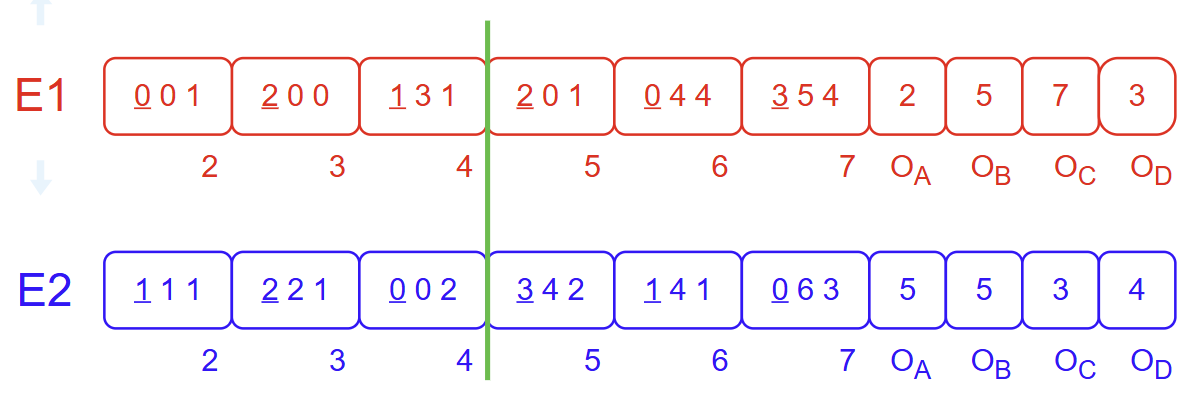
\includegraphics[scale = 0.45]{Bilder/BeispielOnePointCrossover.png}
    \caption{Eltern-Chromosomen One-Point Rekombination, angelehnt an \cite{torabi_using_2022}}
    \label{fig:onePointCrossoverEltern}
\end{figure}

Das erste Eltern-Chromosom (E1, rot) in diesem Beispiel wurde aus Abbildung \ref{fig:genotyp} entnommen.
Das zweite Eltern-Chromosom (E2, blau) ist ein zufällig gewähltes Beispielchromosom.\\
Bei beiden Chromosomen wird vorerst nicht weiter betrachtet, ob die Knoten aktiv oder inaktiv sind, da sich dieses Merkmal mit der Rekombination und Mutation ändern kann.
Angenommen wird, dass C1 und C2 aus der letzten Generation übernommen wurden, da sie die beste Fitness aufgewiesen haben.\\
Für die One-Point Rekombination wird zuerst eine zufällige Stelle innerhalb der Eltern-Chromosomen bestimmt.
Diese ist in Abbildung \ref{fig:onePointCrossoverEltern} grün markiert.
Die Eltern-Chromosomen werden anschließend an dieser Stelle geteilt und überkreuzt zusammengesetzt.
Für dieses Beispiel ergeben sich die beiden folgenden Nachwuchs-Chromosomen:

\begin{figure}[H]
    \centering
    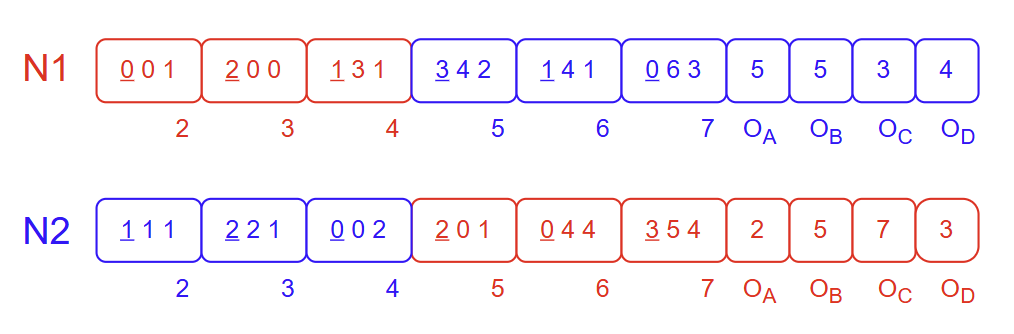
\includegraphics[scale = 0.5]{Bilder/BeispielOnePointCrossover2.png}
    \caption{Nachwuchs-Chromosomen One-Point Rekombination, angelehnt an \cite{torabi_using_2022}}
    \label{fig:onePointCrossoverNachwuchs}
\end{figure}

\subsection{Two-Point Rekombination}
\label{subsubsec:twoPointCrossover}

Für die Grundlagen dieses Abschnitts wurde \cite{pavai_survey_2017} als Quelle verwendet.\\
Das Verfahren der Two-Point Rekombination funktioniert identisch zur in Abschnitt \ref{subsubsec:onePointCrossover} erläuterten One-Point Rekombination, mit dem Unterschied, dass zwei zufällige Stellen ausgewählt werden, an denen die Chromosomen geteilt werden.\\
Anhand des nachfolgenden Beispiels kann dies nachvollzogen werden:

\begin{figure}[H]
    \centering
    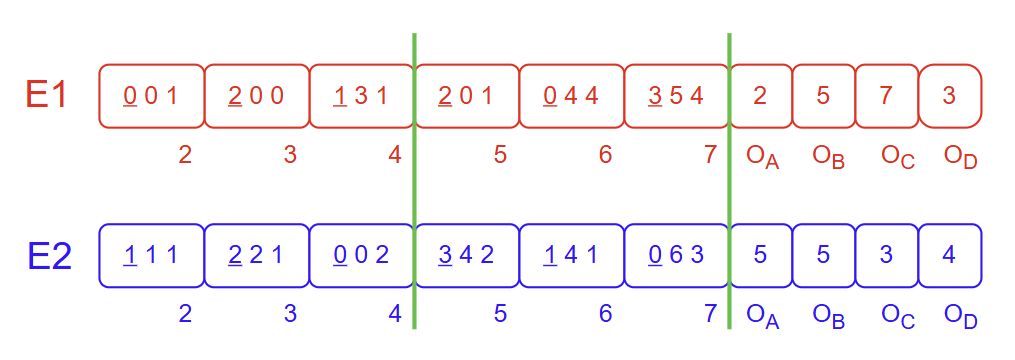
\includegraphics[scale = 0.5]{Bilder/BeispielTwoPointCrossover.png}
    \caption{Eltern-Chromosomen Two-Point Rekombination, angelehnt an \cite{torabi_using_2022}}
    \label{fig:twoPointCrossoverEltern}
\end{figure}
\begin{figure}[H]
    \centering
    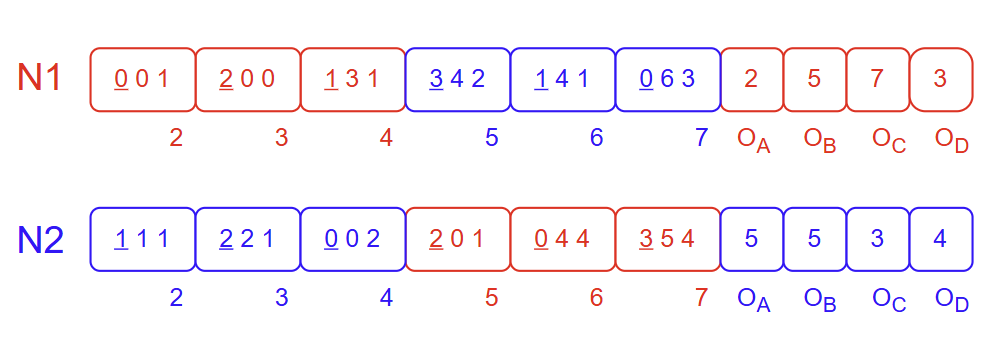
\includegraphics[scale = 0.5]{Bilder/BeispielTwoPointCrossover2.png}
    \caption{Nachwuchs-Chromosomen Two-Point Rekombination, angelehnt an \cite{torabi_using_2022}}
    \label{fig:twoPointCrossoverNachwuchs}
\end{figure}

Zu beobachten ist, dass die Eltern-Chromosomen an jeweils zwei Stellen aufgeteilt werden (grün).
Die Nachwuchs-Chromosomen bilden sich anschließend abwechselnd aus den Teilstücken der beiden Eltern-Chromosomen.
In der Abbildung wird dieser Prozess deutlich, indem die Chromosomenteile des ersten Elternteils rot markiert sind und des zweiten blau.


\subsection{Uniform Rekombination}
\label{subsubsec:unformCrossover}
Die Erläuterung der Uniform Rekombination basiert auf \cite{syswerda_uniform_1989}.\\
Was die Uniform Rekombination von der One-Point oder Two-Point Rekombination abhebt, ist die Verwendung einer Maske. 
Die Maske ist genauso lang wie die Eltern-Chromosomen und beinhaltet für jede Stelle binäre Werte.
Diese Werte geben jeweils an, von welchem Elternteil die jeweilige Stelle im Chromosom des Nachwuchses stammen soll.
Der zweite gebildete Nachwuchs bekommt in diesem Prozess das Gen des jeweils anderen Elternteils.\\
Anhand der Abbildungen \ref{fig:uniformCrossoverEltern} und \ref{fig:uniformCrossoverNachwuchs} lässt sich die Uniform Rekombination beispielhaft erklären:

\begin{figure}[H]
    \centering
    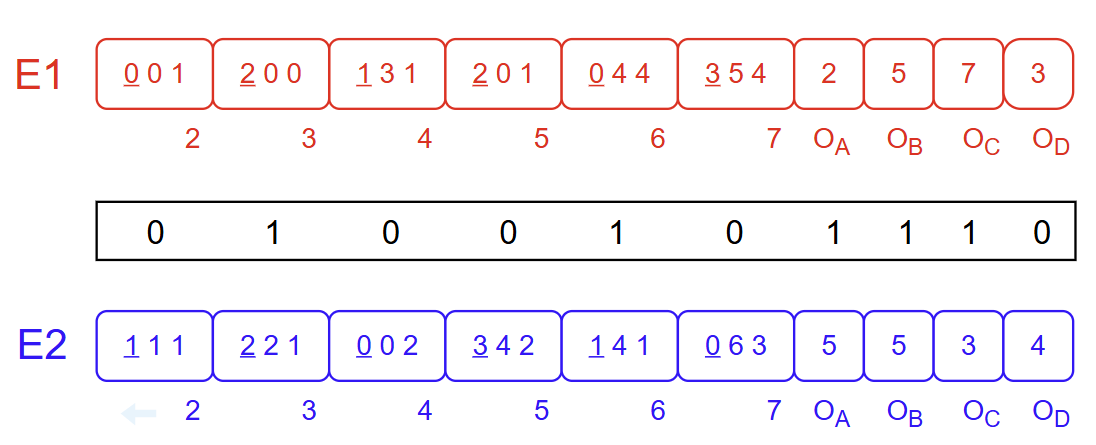
\includegraphics[scale = 0.45]{Bilder/BeispielUniformCrossover.png}
    \caption{Eltern-Chromosomen Uniform Rekombination, angelehnt an \cite{torabi_using_2022}}
    \label{fig:uniformCrossoverEltern}
\end{figure}

Abbildung \ref{fig:uniformCrossoverEltern} zeigt die Ausgangssituation mit den beiden Eltern-Chromosomen (E1 und E2) in rot und blau.
Zwischen den beiden Eltern-Chromosomen wird schwarz die Maske angezeigt.
Diese wird zufällig binär gefüllt, bis sie die Länge der beiden Eltern-Chromosomen erreicht.\\
Im folgenden Schritt werden die Nachwuchs-Chromosomen anhand der Maske erzeugt.
Der entsprechende Index des Knotens kann jeweils unterhalb der Eltern-Chromosomen abgelesen werden.
Für den ersten Wert der Maske ergibt das den Knotenindex 2.
In diesem Beispiel enthält der erste Wert der Maske eine 0.
Dementsprechend wird für den Knoten mit dem Index 2 des ersten Nachwuchs-Chromosoms (N1) der jeweilige Knoten des ersten Eltern-Chromosoms (E1, rot) verwendet.
Das zweite Nachwuchs-Chromosom (N2) bekommt demnach den entsprechenden Knoten aus dem zweiten Eltern-Chromosom (E2, blau).\\
Für den darauffolgenden Index hat die Maske den Wert 1.
Dies bedeutet, dass die Vererbungen genau andersherum ablaufen: N1 bekommt den Knoten von E2 und N2 bekommt den Knoten von E1.
Dieser Prozess wird für alle Indices ausgeführt.
Die folgende Abbildung zeigt die resultierenden Ergebnisse für dieses Beispiel der Uniform Rekombination.

\begin{figure}[H]
    \centering
    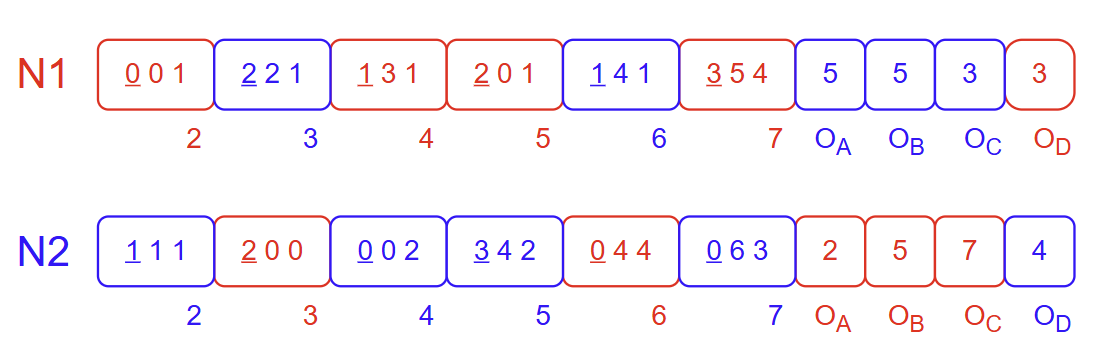
\includegraphics[scale = 0.45]{Bilder/BeispielUniformCrossover2.png}
    \caption{Nachwuchs-Chromosomen Uniform Rekombination, angelehnt an \cite{torabi_using_2022}}
    \label{fig:uniformCrossoverNachwuchs}
\end{figure}


\subsection{Rekombinationsraten}

In den letzten Abschnitten wurden unterschiedliche Rekombinationsalgorithmen erläutert.
Der Rekombinationsschritt wird allerdings nicht für jedes Nachwuchs-Chromosom verwendet.
Dieser wird nur zu einer bestimmten Wahrscheinlichkeit ausgeführt, welche mit der Rekombinationsrate beschrieben wird.
Die Effektivität des (C)GP-Systems hängt unter anderem von der richtigen Wahl der Rekombinationsrate ab. \cite{hassanat_choosing_2019}\\
Um das bestmögliche (C)GP-System zu erhalten, sollte das richtige Verhältnis aus Exploration (dt. Erforschung) und Exploitation (dt. Ausbeutung) des Lösungsraums erzielt werden. 
Exploration ist dabei der Prozess, neue Bereiche des Lösungsraums zu erkunden, während bei der Exploitation bereits erkundete Regionen des Lösungsraums näher betrachtet werden.
Eine Stellschraube, um den eigenen Prozess dahingehend zu steuern, ist die Rekombinationsrate. \cite{crepinsek_exploration_2013}
Wird die Rekombinationsrate sehr hoch eingestellt, wird zu einem hohen Maß Exploration betrieben. 
Dies führt allerdings dazu, dass die Exploitation niedrig gehalten wird und somit die optimalen Lösungen verfehlt werden. \cite{pavai_survey_2017}\\
In unterschiedlichen Papern werden verschiedene Herangehensweisen vorgeschlagen, diesen Parameter zu wählen.
Teilweise widersprechen sich diese Aussagen.
Ziel dieser Arbeit ist es, unter anderem einen Einblick zu bekommen, wie man die Rekombinationsrate richtig wählen kann und welche Auswirkungen sie auf die Güte von CGP-Lösungen hat.\\

Die folgenden Abschnitte geben einen Einblick über die unterschiedlichen Möglichkeiten, die Rekombinationsrate zu belegen.

\subsubsection{Konstante Rekombinationsrate}
\label{subsubsec:konstanteCrossover}

Wie von Hassanat et al. beschrieben, ist die konstante (statische) Rekombinationsrate die übliche Form. 
Als geläufiges Beispiel wird in ihrem Paper der Wert 0,9 für die Rekombinationsrate vergeben. \cite{hassanat_choosing_2019} 
Dies bedeutet, dass zur Initialisierung des CGP ein fester Wert für die Rekombinationsrate gewählt wird.
Dieser gilt für alle Generationen gleichermaßen und wird nicht verändert.\\
Diese \glqq klassische\grqq Form der Rekombination kann in der Evaluation der praktischen Tests dazu verwendet werden, um die erste Forschungsfrage zu beantworten.
Durch diese einfachste Form der Rekombinationsrate kann überprüft werden, ob CGPs ohne oder mit (klassischer) Rekombination effizienter sind.\\
Mit Hilfe der in den nächsten Abschnitten folgenden Anpassungen der Rekombinationsrate kann anschließend überprüft werden, ob die Effizienz von CGP mit Rekombination weiter verbessert werden kann.

\subsubsection{Linear fallende Rekombinationsrate}
\label{subsubsec:CleggCrossover}

Clegg et al. präsentieren in ihrem Paper aus 2007 eine neue Form der Rekombination.
Dabei treffen sie auch einige Aussagen über die Rekombinationsrate, die in diesem Abschnitt näher betrachtet werden sollen.\cite{clegg_new_2007}\\
Sie beobachten, dass sich für höhere Rekombinationsraten eine schnellere Konvergenz der Fitness innerhalb der ersten Generationen einstellt.
Gleichzeitig stellen sie fest, dass in ihrem Beispiel ab der 200. Generation Rekombination keinen signifikanten Vorteil mehr in der Performance liefert.\\
Aus diesen beiden Beobachtungen konstruieren sie eine neue, dynamische Rekombinationsrate.
Diese beginnt bei einem hohen Startwert von 0,9 und sinkt linear, bis eine Rekombinationsrate von 0,0 erreicht wird. 
In ihrem Beispiel legen sie über händische Analysen eine Generation fest, bis zu welcher die Rekombinationsrate auf 0,0 fallen soll.\\
Innerhalb des praktischen Teils dieser Arbeit wird 0,9 für den Startwert der Rekombinationsrate übernommen, um die Anzahl der Parameter in der Hyperparameteranalyse zu reduzieren.
Ebenfalls ist es ein Vorteil, nur einen variablen Parameter pro Rekombinationsraten-Typ zu verwenden, da gegebenenfalls die Änderungen innerhalb der Ergebnisse für die verschiedenen Parameter besser miteinander verglichen werden können.\\
Der einzige variable Parameter für die linear fallende Rekombinationsrate ist in dieser Arbeit die Rate, die nach jeder Generation von der alten Rekombinationsrate abgezogen werden soll, um die neue Rekombinationsrate zu erhalten.

\subsubsection{One-Fifth-Regel angewandt auf die Rekombinationsrate}
\label{subsubsec:oneFifthCrossover}

Die One-Fifth-Regel gibt es bereits andere Parameter von GP, wie beispielsweise für die Mutationsrate.
Diese wird ebenfalls im Paper von Milano und Nolfi verwendet.
Dabei handelt es sich um einen Weg, die Mutationsrate automatisch und dynamisch an die Problemcharakteristiken und die evolutionäre Phase anzupassen. \cite{milano_scaling_2018}\\
Betrachtet wird bei dieser Regel das Fitness-Verhältnis der Elitisten und der neuen Chromosomen.
In anderen Worten werden die Kinder also mit ihren Eltern verglichen.
Erzielt werden soll ein Verhältnis von 20\%.
Das heißt, dass 20\% der Nachwuchs-Chromosomen eine bessere Fitness aufweisen sollen als ihre Eltern.
Wird dieses Verhältnis unter- oder übertroffen, wird der jeweilige Parameter verkleinert oder vergrößert. \cite{doerr_self-adjusting_2019}\\

In dieser Arbeit soll die One-Fifth-Regel für die dynamische Anpassung der Rekombinationsrate herangezogen werden.
Um nur den Rekombinationsschritt zu bewerten und nicht den Mutationsschritt, muss die Bewertung der Fitness vor der Mutation geschehen.
Dementsprechend wird für die One-Fifth-Regel in dieser Arbeit direkt nach dem Rekombinationsschritt die Fitness der Eltern- mit der Fitness der Nachwuchs-Chromosomen verglichen.
Anschließend wird betrachtet, ob 20\% der Kinder eine bessere Fitness aufweisen als ihre Eltern.
Wird dieser Wert übertroffen, wird die Rekombinationsrate mit 1,1 multipliziert, um den Erfolg des Rekombinationsschritts auszuschöpfen.
Andernfalls wird die Rekombinationsrate mit 0,9 multipliziert und somit verringert.


\subsubsection{Rekombinationsrate mit Offset}
\label{subsubsec:offsetCrossover}
Torabi et el. beschreiben in ihrem Paper eine neue Rekombinationsstrategie \cite{torabi_using_2022}.
Dabei verwenden sie einen Hyperparameter, der den Offset der Rekombination definieren soll.
Das heißt, dass die Rekombination in ihrer Strategie in den ersten Generationen nicht angewendet wird, sondern erst zu einer bestimmten Generation beginnt.
Wie dieser Hyperparameter bestimmt wurde und welche Größenordnung dieser einhalten sollte, wird in dem Paper allerdings nicht erwähnt.\\

Torabi et al. behaupten außerdem, dass ihre Strategie \glqq den richtigen Kompromiss aus Exploration und Exploitation\grqq\space erreicht.
Vergleicht man diese Aussage mit der Aussage von Clegg et al., stellt man fest, dass sich diese Aussagen widersprechen \cite{clegg_new_2007}:
Während Clegg et al. vor allem in den ersten Generationen auf Rekombination setzen, da der Rekombinationsschritt hier zu einer höheren Fitness-Konvergenz führen soll, meiden Torabi et al. in ihrer Strategie Rekombinationen in den ersten Generationen völlig.\\
Ein Ziel dieser Arbeit ist es herauszufinden, ob sich ein Offset in der Rekombination als sinnvoll erweist oder ob sich dieser nur für die Rekombinationsstrategie eignet, die Torabi et al. in ihrem Paper eingeführt haben.


\section{Evolutionärer Operator: Mutation}
\label{subsec:Mutation}

TODO: Mutation grundlegend erklären mit Shift-Operator

TODO: wegen single active mutation keine Mutationsrate -> Exploration und Exploitation Verhalten liegt rein an Rekombinationsrate


\begin{itemize}
    \item Grundsätzliches Vorgehen über Generationen hinweg (anhand von GP erklären und dann Unterschied zu CPG erklären): Grafik -> \glqq Genetic Programming Principles and Applications\grqq
    \item Aufbau des Graphen
    \item Wozu CGP? Welche Probleme können damit gelöst werden? -> aus Eingabe(n) eine oder mehrere Ausgabe(n) generieren
    \item Arten von Knoten
    \item aktive und inaktive Knoten
    \item Exploration vs Exploitation
    \item Selektion
    \begin{itemize}
        \item Ziel Selektion grundsätzlich
        \item neutral search
        \item Elitisten (Was ist das und Sinn)
        \item mu lambda
        \item ggf tournament
    \end{itemize}
    \item Rekombination
    \begin{itemize}
        \item Single-point
        \item two-point
        \item uniform
        \item Rekombinationsraten
        \begin{itemize}
            \item Ziel: Geeignetes Maß an Exploration vs Exploitation finden
            \item Clegg et al
            \item Torabi et al
            \item One-Fifth Rule der Mutationsrate
        \end{itemize}
    \end{itemize}
    \item Mutation
    \begin{itemize}
        \item Mutation grundsätzlich
        \item single active mutation -> Mutationsrate nicht betrachtet (weniger Parameter in HPO)
    \end{itemize}
    \item Hyperparameter analysis -> Sampler
    \item ANOVA
\end{itemize}

\chapter{Experimente und Evaluation}
\label{praktischer Teil}

\section{Aufbau der Experimente}
\label{sec:aufbauExperimente}

Für die Beantwortung der Forschungsfragen werden unterschiedliche Experimente ausgeführt, deren Ergebnisse in dieser Arbeit ausgewertet und interpretiert werden sollen.
Der Programmcode für die Experimente wurde in der Sprache Julia verfasst.
Dabei fand eine Orientierung an folgendem Code von Henning Cui statt: \cite{cuihen_cuihencgp_with_crossover_strategies_2024}\\
Um Ergebnisse von Ausgangsproblemen aus unterschiedlichen Domänen für eine umfangreichere Bewertung zur Verfügung zu stellen, werden mehrere Benchmark-Testszenarien überprüft.
Diese werden in den folgenden Abschnitten näher betrachtet.

\subsection{Testszenarien}
\label{subsec:testszenarien}

\subsubsection{Boolean Problems}
\label{subsubsec:booleanProblems}

Nach der Aussage von Kalkreuth et al. spielen Boolean Problems eine wichtige Rolle in der Forschung zu GP.
Grundsätzlich ist bei Boolean Problems das Ziel einen sinnvollen Zusammenhang zwischen Ein- und Ausgaben zu generieren, welcher von Boolean Funktionen bestimmt wird.
Diese können wiederum durch Boolean Ausdrücke mathematisch beschrieben werden.
Die verschiedenen Boolean Funktionen können durch Wahrheitstabellen dargestellt werden, in denen die jeweiligen Ein- und Ausgaben miteinander verknüpft werden. \cite{kalkreuth_towards_2023}
Das Ziel von CGP-Algorithmen ist es aus Eingängen die richtigen Ausgänge zu generieren, welche dem Mapping der Boolean Funktionen entsprechen.\\

Insgesamt werden in dieser Arbeit vier Boolean Benchmark Problems für die Evaluation der CGP Algorithmen betrachtet: 3-bit Parity, 16-4-bit Encode, 4-16-bit Decode und 3-bit Multiply (vereinfacht bezeichnet als Parity, Encode, Decode und Multiply).
Die Auswahl dieser beruht auf der Argumentationskette von Cui et al., die für sinnvoll befunden wird. \cite{cui_equidistant_2023}\\
Obwohl Parity als zu leichtes Ausgangsproblem für GP bezeichnet wird \cite{white_better_2013}, wird es häufig als Benchmarkproblem genutzt \cite{yu_neutrality_2001, kaufmann_kalkreuth_2017, kaufmann_kalkreuth_2020}.
Um Benchmarkprobleme mit unterschiedlichen Ein- und Ausgangsgrößen miteinzubeziehen, werden Encode und Decode verwendet.
Sinnvoll ist es ebenfalls Testprobleme verschiedener Schwierigkeitsstufen zu bewerten.
Multiply ist dabei ein vergleichsweise schwer zu lösendes Testproblem und wird deswegen herangezogen \cite{walker_2008}.\\

Das verwendete Standardfunktionsset aller vier Testszenarien beinhaltet die Boolean Rechenoperatoren AND, OR, NAND und NOR.
Außerdem wird die Standardfitnessfunktion für Boolean Benchmarkprobleme verwendet.
Diese wird definiert durch den Anteil an korrekt zugeordneten Bits. \cite{cui_equidistant_2023}
Folgend werden die vier verwendeten Boolean Benchmark Problems näher erläutert:

\textbf{Parity:} N-bit Parity ist eine Mapping-Funktion, die angibt, ob die Summe der Komponenten eines Binär-Vektors gerade oder ungerade ist.
Bei 3-bit Parity handelt es sich dabei um Binär-Vektoren der Länge 3.
Das Evaluationsset besteht aus $2^N=2^3$ Testvektoren. \cite{hohil_1999}
Demnach gibt es für das CGP drei Eingaben (die Komponenten eines Binär-Vektors) und eine Ausgabe (Binärwert für \glqq gerade\grqq\space / \glqq ungerade\grqq).

\textbf{Encode:} Beim 16-4-bit Encoding wird aus einer 16-stelligen One-Hot-Kodierung ein 4-bit Integer erstellt.
Die One-Hot-Kodierung besteht dabei aus einem 16-stelligen Binär-Vektor, wobei nur eine Stelle mit einer 1 belegt ist, die restlichen Stellen sind 0.
Ziel ist es diejenige Stelle zu finden, die die 1 hält und diese als üblichen 4-bit Integer zu kodieren. \cite{cui_weighted_mutation, goldman_2015}
Daraus ergibt sich eine Eingabegröße von 16 und eine Ausgabegröße von vier.
Der Testdatensatz enthält 16 verschiedene One-Hot-Kodierungen, die umgewandelt werden sollen.

\textbf{Decode:} 4-16-bit Decode hat das genau umgekehrte Ziel als 16-4-bit Encode.
Es wird ein 4-bit Integer-Wert angegeben, der durch eine 16-bit One-Hot-Kodierung dargestellt werden soll. \cite{cui_weighted_mutation}
Demnach werden für 4-16-bit Decode vier Eingaben in 16 Ausgaben umgewandelt.
Der Testdatensatz besteht aus 16 verschiedenen 4-bit Integerwerten.

\textbf{Multiply:} Ziel von 3-bit Multiply ist die Multiplikation von zwei 3-bit Integer-Werten.
Das Ergebnis wird durch einen 6-bit Integer-Wert dargestellt. \cite{cui_weighted_mutation}
Folglich ist die Anzahl der CGP-Eingaben gleich 6, da beide 3-bit Faktoren als Eingang in das CGP-Modell einfließen müssen.
Für die Ausgabe werden ebenfalls 6 Binärausgaben benötigt.
Der Testdatensatz besteht aus $2^6=64$ verschiedenen Kombinationen der möglichen Binär-Faktoren.

\subsubsection{Symbolische Regression}
\label{subsubsec:symbolicRegression}

\section{Evaluation}
\label{sec:Evaluation}

\begin{itemize}
    \item Versuchsaufbau und Durchführung
    \begin{itemize}
        \item an Hennings Code orientiert
        \item Testszenarien -> welche Testdaten und Berechnung fitness
        \begin{itemize}
            \item boolean Problems
            \item symbolic regression
            \item ggf. Ameisenoptimierungsproblem
        \end{itemize}
        \item weitere Einstellungen (Welche Selektionsverfahren, Mutationsverfahren, Rekomb...)
        \item Hyperparameteroptimierung
        \begin{itemize}
        	\item HPO wird in Grundlagen nicht erklärt also hier kurz erwähnen, dass die besten Parameter gesucht werden also eine HPO ausgeführt wird
            \item Welche Bib benutzt
            \item Welche Parameter optimiert; mit welchen Ranges
            \item 10 Ausführungen pro Optimierungsschritt
            \item Probleme Rechenzeit HPO
            \item verschiedene Sampler keinen Mehrwert
        \end{itemize}
        \item Ausführen mehrerer Durchläufe, um statistische Auswertung vorzunehmen
    \end{itemize}
    \item Ergebnisse und Evaluation
    \begin{itemize}
        \item Metriken zur Auswertung
        \item händische Auswertung des zeitlichen Verlaufs der Metriken (Mittelwert und Standardabweichung)
        \item bayesian Auswertung der Endergebnisse -> wie viele Iterationen (erklären wieso Bayes verwendet wird: Henning sagt in Paper, dass andere Verteilungen das Modell nicht gut beschreiben; siehe negative Werte für Iterationen)
        \item Plankett-Luce-Modell gibt Wahrscheinlichkeit bestes Ergebnis zu sein -> wie in Hennings Paper
        \item cmpbayes verwendet Markov Chain Monte-Carlo Sampling -> also auch verwenden
        \item HPDI für Bewertung der Endergebnisse (Iterationen bis konvergent)
        \item prior sensitivity analysis nicht machen (to ensure robustness of all models)
        \item ggf Bewertung der statistischen Aussagekraft mit ANOVA
    \end{itemize}
\end{itemize}


\chapter{Ergebnisse}
\label{Ergebnisse}
Ergebnisse

TODO: Argumentation, dass Offset nicht so viel bringt (damit Kapitel \glqq praktischer Teil\grqq\space darauf verweisen kann)\\
- HPO: mehrere Durchläufe wählen garkeinen Offset\\
- restliche Tests vergleichen zwischen mit Offset und ohne

\section{Ergebnisse: Boolesche Probleme}
\label{sec:ergebnisseBP}

\subsection{Ergebnisse: Parity}
\label{subsec:ergebnisseParity}
\subsubsection{Analyse der Rohdaten}
\label{parity:analyseRohdaten}

\begin{table}[H]
	\centering
	\begin{tabular}{c | c | c | c | c | c }
		\begin{turn}{270} \textbf{CGP-Konfigurationen} \end{turn} & \begin{turn}{270} \textbf{Anzahl pos. Mutationen} \end{turn} & \begin{turn}{270} \textbf{Anzahl pos. Rekomb.} \end{turn} & \begin{turn}{270} \textbf{Anzahl neg. Mutationen} \end{turn} & \begin{turn}{270} \textbf{Median Iter. pos. Rekomb.} \end{turn} & \begin{turn}{270} \textbf{Median Iter. bis Konv.} \end{turn}\\
		\hline
		keine Rekomb. & 133 & 0 & 0 & - & 58.5\\
		\hline
		One-Point Konstant kein Offset & 126 & 8 & 2 & 5.5 & 44.0\\
		\hline
		One-Point Konstant mit Offset & 136 & 0 & 0 & - & 49\\
		\hline
		One-Point Clegg kein Offset & 123 & 13 & 3 & 4 & 74\\
		\hline
		One-Point Clegg mit Offset & 126 & 0 & 0 & - & 43.5\\
		\hline
		One-Point OneFifth kein Offset & 116 & 2 & 1 & 2.0 & 37.0\\
		\hline
		One-Point One-Fifth mit Offset & 127 & 0 & 0 & - & 27.5\\
		\hline
		Two-Point Konstant kein Offset & 108 & 10 & 2 & 3.0 & 33.5\\
		\hline
		Two-Point Konstant mit Offset & 129 & 0 & 0 & - & 64\\
		\hline
		Two-Point Clegg kein Offset & 106 & 20 & 8 & 6.5 & 40.0\\
		\hline
		Two-Point Clegg mit Offset & 125 & 0 & 0 & - & 70.5\\
		\hline
		Two-Point OneFifth kein Offset & 126 & 4 & 2 & 3.0 & 59.5\\
		\hline
		Two-Point OneFifth mit Offset & 125 & 0 & 0 & - & 43\\
		\hline
		Uniform Konstant kein Offset & 85 & 44 & 15 & 14.0 & 55\\
		\hline
		Uniform Konstant mit Offset & 131 & 0 & 0 & - & 37.5\\
		\hline
		Uniform Clegg kein Offset & 101 & 41 & 15 & 4 & 31\\
		\hline
		Uniform Clegg mit Offset & 130 & 0 & 0 & - & 51.5\\
		\hline
		Uniform OneFifth kein Offset & 108 & 22 & 12 & 5.0 & 69.5\\
		\hline
		Uniform OneFifth mit Offset & 123 & 0 & 0 & - & 54.0\\
	\end{tabular}
	\caption{Parity: Auswertung der Rohdaten}
	\label{table:parityRohdaten}
\end{table}

\subsubsection{Bayes'sche Analyse}
\label{parity:bayes}
\subsubsection{Graphische Evaluation}
\label{parity: graphische Evaluation}

\subsection{Ergebnisse: Encode}
\label{subsec:ergebnisseEncode}
\subsubsection{Analyse der Rohdaten}
\label{encode:analyseRohdaten}
\subsubsection{Bayes'sche Analyse}
\label{encode:bayes}
\subsubsection{Graphische Evaluation}
\label{encode: graphische Evaluation}


\subsection{Ergebnisse: Decode}
\label{subsec:ergebnisseDecode}
\subsubsection{Analyse der Rohdaten}
\label{decode:analyseRohdaten}
\subsubsection{Bayes'sche Analyse}
\label{decode:bayes}
\subsubsection{Graphische Evaluation}
\label{decode: graphische Evaluation}

TODO: ggf mehr Testprobleme einfügen

\section{Ergebnisse: Symbolische Regression}
\label{sec:ergebnisseSR}

\subsection{Ergebnisse: Keijzer}
\label{subsec:ergebnisseKeijzer}
\subsubsection{Analyse der Rohdaten}
\label{keijzer:analyseRohdaten}

\begin{table}[H]
	\centering
	\begin{tabular}{c | c | c | c | c | c }
		\begin{turn}{270} \textbf{CGP-Konfigurationen} \end{turn} & \begin{turn}{270} \textbf{Anzahl pos. Mutationen} \end{turn} & \begin{turn}{270} \textbf{Anzahl pos. Rekomb.} \end{turn} & \begin{turn}{270} \textbf{Anzahl neg. Mutationen} \end{turn} & \begin{turn}{270} \textbf{Median Iter. pos. Rekomb.} \end{turn} & \begin{turn}{270} \textbf{Median Iter. bis Konv.} \end{turn}\\
		\hline
		keine Rekomb. & 2260 & 0 & 0 & - & 624\\
		\hline
		One-Point Konstant kein Offset & 1183 & 26 & 16 & 13.0 & 756\\
		\hline
		One-Point Konstant mit Offset & 1531 & 0 & 0 & - & 374.0\\
		\hline
		One-Point Clegg kein Offset & 1584 & 59 & 28 & 5 & 243\\
		\hline
		One-Point Clegg mit Offset & 1534 & 0 & 0 & - & 396.5\\
		\hline
		One-Point OneFifth kein Offset & 1307 & 35 & 18 & 3 & 766.0\\
		\hline
		One-Point One-Fifth mit Offset & 1776 & 0 & 0 & - & 229.0\\
		\hline
		Two-Point Konstant kein Offset & 1854 & 79 & 25 & 15 & 803.0\\
		\hline
		Two-Point Konstant mit Offset & 1361 & 0 & 0 & - & 548\\
		\hline
		Two-Point Clegg kein Offset & 1467 & 106 & 62 & 18.5 & 735\\
		\hline
		Two-Point Clegg mit Offset & 1862 & 0 & 0 & - & 201.0\\
		\hline
		Two-Point OneFifth kein Offset & 1788 & 17 & 10 & 4 & 753\\
		\hline
		Two-Point OneFifth mit Offset & 1124 & 0 & 0 & - & 158.0\\
		\hline
		Uniform Konstant kein Offset & 1224 & 480 & 239 & 24.0 & 363\\
		\hline
		Uniform Konstant mit Offset & 1890 & 0 & 0 & - & 260.5\\
		\hline
		Uniform Clegg kein Offset & 1386 & 77 & 57 & 6 & 723\\
		\hline
		Uniform Clegg mit Offset & 2232 & 0 & 0 & - & 385.5\\
		\hline
		Uniform OneFifth kein Offset & 1491 & 106 & 50 & 8.0 & 155\\
		\hline
		Uniform OneFifth mit Offset & 1749 & 0 & 0 & - & 445.5\\
	\end{tabular}
	\caption{Keijzer: Auswertung der Rohdaten}
	\label{table:keijzerRohdaten}
\end{table}

\subsubsection{Bayes'sche Analyse}
\label{keijzer:bayes}
\subsubsection{Graphische Evaluation}
\label{keijzer: graphische Evaluation}


\subsection{Ergebnisse: Koza}
\label{subsec:ergebnisseKoza}
\subsubsection{Analyse der Rohdaten}
\label{koza:analyseRohdaten}
\subsubsection{Bayes'sche Analyse}
\label{koza:bayes}
\subsubsection{Graphische Evaluation}
\label{koza: graphische Evaluation}

TODO: ggf mehr Testprobleme einfügen

\section{Zusammenfassung der Ergebnisse}
\label{sec:zusammenfassungErgebnisse}

\chapter{Fazit aus Ausblick}
\label{Fazit}

Da das klassische GP bereits in verschiedenen Domänen für Problemlösungen verwendet wird, ist es sinnvoll den Bereich des CGP näher zu betrachten.
Laut Miller werde der Rekombinationsschritt in CGPs normalerweise nicht ausgeführt, da dieser die Effizienz eines CGP-Modells nicht zielführend steigert \cite{miller_cartesian_2020}.
Trotzdem wäre es sinnvoll neben der Mutation einen weiteren genetischen Operator einzubinden, um die Effizienz des CGPs zu steigern und somit komplexere Ausgangsprobleme lösbar zu machen.
Die Aussagen, dass Rekombinationsschritte bisher nicht sinnvoll in das Standard-CGP eingepflegt werden können basiert auf Papern von Miller aus den Jahren 1999 und 2011.
Diese Aussage wird in dieser Arbeit erneut überprüft.
Da der Erfolg der Rekombination stark von der Wahl der Rekombinationsrate abhängt, werden in dieser Arbeit ebenfalls unterschiedliche Arten für Rekombinationsraten betrachtet und bewertet.
Für diese Arbeit ergeben sich demnach die folgenden zwei Forschungsfragen:\\
1. Kann mit heutigem Forschungsstand nachgewiesen werden, dass Rekombination in Standard-CGP sinnvoll eingesetzt werden kann im Vergleich zu CGP ohne Rekombinationsschritt?\\
2. Hat die Art und Weise der Rekombinationsratenberechnung eine Auswirkung auf die Effektivität des CGPs?

Für die Beantwortung der Forschungsfragen wurden vier verschiedene Testprobleme aufgebaut, die durch CGP-Modelle mit verschiedenen Konfigurationen gelöst werden sollten.
Die verschiedenen CGP-Konfigurationen beinhalteten unterschiedliche Rekombinationsarten Var,ianten der Rekombinationsratenberechnung, sowie die völlige Abwesenheit des Rekombinationsschritts.
Bei zwei der vier Testszenarien wurde eine Hyperparameteranalyse durchlaufen, um die Effizienz der besten Ergebnisse für jede CGP-Konfiguration miteinander zu vergleichen.
Für die anderen zwei Testfälle wurden die Rekombiantionsraten-Arten facettenreich parametriert, um bewerten zu können, wie sich die Parametrierung der Rekombinationsraten auf die Effizienz des CGPs auswirken.\\
Für die Analyse der Ergebnisse wurden zwei unterschiedliche Verfahren angewendet.
Einerseits wurden die aufgezeichneten Rohdaten der Testdurchläufe näher analysiert, andererseits wurde eine Bewertung mit Hilfe der bayes'schen Analyse ausgeführt.\\
TODO: Ergebnisse Arbeit hier einfügen + dazugehörige offene Fragen (danach dann bewertet, ob offene Fragen weiter runter kommen sollen oder hier oben Sinn machen)

Zusammenfassend lassen sich die zwei Forschungsfragen wie folgt beantworten:\\
In Standard-CGPs kann Rekombination durchaus sinnvoll eingesetzt werden.
Dafür ist es allerdings relevant die richtige Parametrierung mit Hilfe einer Hyperparameteranalyse zu ermitteln.
Teil dieser Analyse sollten ebenfalls die Wahl der richtigen Rekombinationsart und Rekombinationsraten-Art sein.
Weiter wurde herausgefunden, dass die Rekombination ein größeres Potential für die Verbesserung der Effizienz des CGPs aufweist, das im Standard-CGP-Verfahren nicht vollständig ausgeschöpft wird.
Hierzu könnten zukünftig weitere Tests ausgeführt werden, um ein geeigneteres CGP-Verfahren zu entwickeln, das Rekombination und Mutation besser vereinen kann.\\
Des weiteren hat die Art und Weise der Rekombinationsratenberechnung einen großen Einfluss auf die Effizienz des CGPs. 
Hohe Rekombinationsraten zu Beginn des Trainings und ein anschließender Abbruch der Rekombination erscheinen besonders sinnvoll.
Zu welcher Iteration die Rekombination im besten Fall ausgesetzt werden soll und ob dies schleichend oder abrupt stattfinden sollte, könnte durch weitere Forschung näher betrachtet werden.




\sloppy
\printbibliography
\fussy


\cleardoublepage


\appendix
\pagenumbering{Roman}
\chapter{Anhang}
\section{Tabellen Rohdatenanalyse}
\label{sec:tablesRohdatenanalyseAppendix}

\subsection{Parity: Tabellen Rohdatenanalyse}

\subsection{Keijzer: Tabellen Rohdatenanalyse}

\subsection{Encode: Tabellen Rohdatenanalyse}

\subsection{Koza: Tabellen Rohdatenanalyse}
TODO: Tabellen einfügen\\
...

\section{Tabellen Bayes'sche Analyse}
\label{sec:appendixTabellenBayes}

\subsection{Parity: Tabelle Bayes'sche Analyse}
\label{subsec:appendixTabelleBayesParity}

\begin{table}[H]
	\centering
	\begin{tabular}{c | c | c | c}
		\textbf{CPG-Konfiguration} & \textbf{HPDI (Iter.)} & \textbf{MW} & \textbf{PL-Platz}\\
		\hline
		Parity keine Rekombination & (237,958; 541,181) & 357,440 & 0,034518\\
		\hline
		Parity One-Point Konstant kein Offset & (72,803; 131,161) & 98,059 & 0,072723\\
		\hline
		Parity One-Point Konstant mit Offset & (117,5867; 241,124) & 168,301 & 0,059872\\
		\hline
		Parity One-Point Clegg kein Offset & (111,330; 204,672) & 151,207 & 0,058134\\
		\hline
		Parity One-Point Clegg mit Offset & (136,755; 318,250) & 208,318 & 0,064637\\
		\hline
		Parity One-Point One-Fifth kein Offset & (305,150; 879,234) & 516,320 & 0,041265\\
		\hline
		Parity One-Point One-Fifth mit Offset & (90,584; 192,603) & 132,238 & 0,072643\\
		\hline
		Parity Two-Point Konstant kein Offset & (161,166; 366,726) & 243,306 & 0,056980\\
		\hline
		Parity Two-Point Konstant mit Offset & (185,680; 398,045) & 271,755 & 0,043839\\
		\hline
		Parity Two-Point Clegg kein Offset & (143,411; 320,218) & 214,015 & 0,055768\\
		\hline
		Parity Two-Point Clegg mit Offset & (279,211; 671,061) & 429,804 & 0,041189\\
		\hline
		Parity Two-Point One-Fifth kein Offset & (165,870; 369,988) & 247,230 & 0,051913\\
		\hline
		Parity Two-Point One-Fifth mit Offset & (187,841; 467,866) & 294,748 & 0,049240\\
		\hline
		Parity Uniform Konstant kein Offset & (182,312; 414,373) & 275,283 & 0,043305\\
		\hline
		Parity Uniform Konstant mit Offset & (158,116; 357,830) & 238,048 & 0,060934\\
		\hline
		Parity Uniform Clegg kein Offset & (120,352; 267,732) & 179,796 & 0,063633\\
		\hline
		Parity Uniform Clegg mit Offset & (147,184; 317,828) & 215,359 & 0,051520\\
		\hline
		Parity Uniform One-Fifth kein Offset & (233,817; 551,718) & 356,681 & 0,040460\\
		\hline
		Parity Uniform One-Fifth mit Offset & (211,377; 519,471) & 329,524 & 0,037426\\
	\end{tabular}
	\label{table:parityBayesian}
	\caption{Parity: Bayes'sche Analyse}
\end{table}


\subsection{Keijzer: Tabelle Bayes'sche Analyse}
\label{subsec:appendixTabelleBayesKeijzer}

\begin{table}[H]
	\centering
	\begin{tabular}{c | c | c | c}
		\textbf{CGP-Konfiguration} & \textbf{HPDI (Iter.)} & \textbf{MW} & \textbf{PL-Platz}\\
		\hline
		Keijzer keine Rekombination & (5446,690; 16772,637) & 9551,657 & 0,046669\\
		\hline
		Keijzer One-Point Konstant kein Offset & (3155,154; 8685,286) & 5214,911 & 0,056954\\
		\hline
		Keijzer One-Point Konstant mit Offset & (5791,946; 19545,587) & 10837,605 & 0,047578\\
		\hline
		Keijzer One-Point Clegg kein Offset & (4055,470; 14388,586) & 7754,999 & 0,053452\\
		\hline
		Keijzer One-Point Clegg mit Offset & (5182,282; 17954,643) & 9757,394 & 0,046700\\
		\hline
		Keijzer One-Point One-Fifth kein Offset & (3746,883; 10479,686) & 6233,279 & 0,050072\\
		\hline
		Keijzer One-Point One-Fifth mit Offset & (4972,228; 16087,780) & 9402,618 & 0,057995\\
		\hline
		Keijzer Two-Point Konstant kein Offset & (4207,924; 13285,672) & 7464,243 & 0,061749\\
		\hline
		Keijzer Two-Point Konstant mit Offset & (3544,144; 10355,412) & 6056,680 & 0,064480\\
		\hline
		Keijzer Two-Point Clegg kein Offset & (5468,641; 17877,607) & 10017,892 & 0,033887\\
		\hline
		Keijzer Two-Point Clegg mit Offset & (4105,772; 13578,136) & 7663,952 & 0,055730\\
		\hline
		Keijzer Two-Point One-Fifth kein Offset & (4408,582; 12408,349) & 7381,426 & 0,053392\\
		\hline
		Keijzer Two-Point One-Fifth mit Offset & (6970,619; 22911,685) & 13432,511 & 0,052018\\
		\hline
		Keijzer Uniform Konstant kein Offset & (8010,603; 23268,991) & 14688,052 & 0,049104\\
		\hline
		Keijzer Uniform Konstant mit Offset & (3406,437; 10751,973) & 6052,727 & 0,069820\\
		\hline
		Keijzer Uniform Clegg kein Offset & (3856,791; 10850,478) & 6440,975 & 0,060934\\
		\hline
		Keijzer Uniform Clegg mit Offset & (6067,492; 20498,984) & 11238,547 & 0,043535\\
		\hline
		Keijzer Uniform One-Fifth kein Offset & (3511,828; 12119,350) & 6587,897 & 0,070569\\
		\hline
		Keijzer Uniform One-Fifth mit Offset & (4025,084; 11844,356) & 6893,370 & 0,025362\\
	\end{tabular}
	\label{table:keijzerBayesian}
	\caption{Keijzer: Bayes'sche Analyse}
\end{table}


\subsection{Encode: Tabellen Bayes'sche Analyse}
\label{subsec:appendixTabellesnBayesEncode}
\begin{table}[H]
	\centering
	\begin{tabular}{c | c | c | c}
		\textbf{CGP-Konfiguration} & \textbf{HPDI (Fitn.)} & \textbf{MW} & \textbf{PL-Platz}\\
		\hline
		Encode keine Rekombination & (0,02727; 0,06853) & 0,04351 & 0,037632\\
		\hline
		Encode One-Point Konstant: 0,125 & (0,02416; 0,06463) & 0,03969 & 0,038324\\
		\hline
		Encode One-Point Konstant: 0,25 & (0,02342; 0,06255) & 0,03837 & 0,042129\\
		\hline
		Encode One-Point Konstant: 0,375 & (0,02216; 0,05684) & 0,036 & 0,051500\\
		\hline
		Encode One-Point Konstant: 0,5 & (0,02581; 0,06657) & 0,04185 & 0,039946\\
		\hline
		Encode One-Point Konstant: 0,625 & (0,02703; 0,06417) & 0,04188 & 0,037295\\
		\hline
		Encode One-Point Konstant: 0,75 & (0,02484; 0,05755) & 0,03791 & 0,043181\\
		\hline
		Encode One-Point Konstant: 0,875 & (0,02311; 0,06519) & 0,03911 & 0,043490\\
		\hline
		Encode One-Point Konstant: 1,0 & (0,02634; 0,06865) & 0,04257 & 0,038647\\
		\hline
		Encode One-Point Clegg: 0,0005 & (0,01874; 0,05612) & 0,03254 & 0,055842\\
		\hline
		Encode One-Point Clegg: 0,0015 & (0,03085; 0,07312) & 0,04756 & 0,033818\\
		\hline
		Encode One-Point Clegg: 0,0025 & (0,03174; 0,07112) & 0,04783 & 0,036098\\
		\hline
		Encode One-Point Clegg: 0,0035 & (0,0259; 0,05957) & 0,03961 & 0,041856\\
		\hline
		Encode One-Point Clegg: 0,0045 & (0,02262; 0,05981) & 0,03682 & 0,048900\\
		\hline
		Encode One-Point Clegg: 0,0055 & (0,02478; 0,06459) & 0,04044 & 0,041741\\
		\hline
		Encode One-Point One-Fifth: 0,125 & (0,02234; 0,06005) & 0,03702 & 0,045181\\
		\hline
		Encode One-Point One-Fifth: 0,25 & (0,02132; 0,06241) & 0,0368 & 0,047502\\
		\hline
		Encode One-Point One-Fifth: 0,375 & (0,02423; 0,05867) & 0,03784 & 0,046065\\
		\hline
		Encode One-Point One-Fifth: 0,5 & (0,01903; 0,05371) & 0,03227 & 0,059094\\
		\hline
		Encode One-Point One-Fifth: 0,625 & (0,02184; 0,0643) & 0,03777 & 0,044798\\
		\hline
		Encode One-Point One-Fifth: 0,75 & (0,02746; 0,06625) & 0,04286 & 0,039122\\
		\hline
		Encode One-Point One-Fifth: 0,875 & (0,02436; 0,05364) & 0,03622 & 0,050632\\
		\hline
		Encode One-Point One-Fifth: 1,0 & (0,02887; 0,06487) & 0,04343 & 0,037210\\
		
	\end{tabular}
	\label{table:encodeOnePointBayesian}
	\caption{Encode One-Point Rekombination: Bayes'sche Analyse}
\end{table}

\begin{table}[H]
	\centering
	\begin{tabular}{c | c | c | c}
		\textbf{CGP-Konfiguration} & \textbf{HPDI (Fitn.)} & \textbf{MW} & \textbf{PL-Platz}\\
		\hline
		Encode keine Rekombination & (0,02727; 0,06853) & 0,04351 & 0,060688\\
		\hline
		Encode Two-Point Konstant: 0,125 & (0,04657; 0,08164) & 0,06176 & 0,034864\\
		\hline
		Encode Two-Point Konstant: 0,25 & (0,0417; 0,08229) & 0,05853 & 0,035661\\
		\hline
		Encode Two-Point Konstant: 0,375 & (0,03172; 0,07007) & 0,04742 & 0,052497\\
		\hline
		Encode Two-Point Konstant: 0,5 & (0,04318; 0,08532) & 0,06094 & 0,034996\\
		\hline
		Encode Two-Point Konstant: 0,625 & (0,03854; 0,07511) & 0,05397 & 0,044939\\
		\hline
		Encode Two-Point Konstant: 0,75 & (0,05211; 0,08389) & 0,06618 & 0,032466\\
		\hline
		Encode Two-Point Konstant: 0,875 & (0,03614; 0,08027) & 0,05438 & 0,041317\\
		\hline
		Encode Two-Point Konstant: 1,0 & (0,03386; 0,07925) & 0,052 & 0,046878\\
		\hline
		Encode Two-Point Clegg: 0,0005 & (0,03588; 0,07852) & 0,05322 & 0,044082\\
		\hline
		Encode Two-Point Clegg: 0,0015 & (0,0457; 0,08078) & 0,06077 & 0,038072\\
		\hline
		Encode Two-Point Clegg: 0,0025 & (0,03801; 0,07255) & 0,05258 & 0,046365\\
		\hline
		Encode Two-Point Clegg: 0,0035 & (0,04651; 0,09123) & 0,06523 & 0,033403\\
		\hline
		Encode Two-Point Clegg: 0,0045 & (0,0321; 0,07079) & 0,04795 & 0,054050\\
		\hline
		Encode Two-Point Clegg: 0,0055 & (0,03634; 0,08965) & 0,0573 & 0,037620\\
		\hline
		Encode Two-Point One-Fifth: 0,125 & (0,04561; 0,08148) & 0,06082 & 0,039357\\
		\hline
		Encode Two-Point One-Fifth: 0,25 & (0,04353; 0,0687) & 0,05485 & 0,046603\\
		\hline
		Encode Two-Point One-Fifth: 0,375 & (0,04642; 0,07558) & 0,05903 & 0,038107\\
		\hline
		Encode Two-Point One-Fifth: 0,5 & (0,03834; 0,07567) & 0,0539 & 0,041795\\
		\hline
		Encode Two-Point One-Fifth: 0,625 & (0,036; 0,07918) & 0,0536 & 0,045416\\
		\hline
		Encode Two-Point One-Fifth: 0,75 & (0,03114; 0,07277) & 0,04805 & 0,052827\\
		\hline
		Encode Two-Point One-Fifth: 0,875 & (0,03244; 0,07634) & 0,05012 & 0,050999\\
		\hline
		Encode Two-Point One-Fifth: 1,0 & (0,03436; 0,07444) & 0,05057 & 0,046998\\
	\end{tabular}
	\label{table:encodeTwoPointBayesian}
	\caption{Encode Two-Point Rekombination: Bayes'sche Analyse}
\end{table}

\begin{table}[H]
	\centering
	\begin{tabular}{c | c | c | c}
		\textbf{CGP-Konfiguration} & \textbf{HPDI (Fitn.)} & \textbf{MW} & \textbf{PL-Platz}\\
		\hline
		Encode keine Rekombination & (0,02727; 0,06853) & 0,04351 & 0,034349\\
		\hline
		Encode Uniform Konstant: 0,125 & (0,02473; 0,06504) & 0,04031 & 0,037538\\
		\hline
		Encode Uniform Konstant: 0,25 & (0,02356; 0,06581) & 0,03963 & 0,038565\\
		\hline
		Encode Uniform Konstant: 0,375 & (0,03039; 0,07186) & 0,047 & 0,033184\\
		\hline
		Encode Uniform Konstant: 0,5 & (0,02241; 0,05759) & 0,03583 & 0,046007\\
		\hline
		Encode Uniform Konstant: 0,625 & (0,02416; 0,05673) & 0,03719 & 0,045744\\
		\hline
		Encode Uniform Konstant: 0,75 & (0,02399; 0,06258) & 0,03882 & 0,047256\\
		\hline
		Encode Uniform Konstant: 0,875 & (0,02203; 0,05148) & 0,03393 & 0,047177\\
		\hline
		Encode Uniform Konstant: 1,0 & (0,022; 0,05696) & 0,03592 & 0,044608\\
		\hline
		Encode Uniform Clegg: 0,0005 & (0,01801; 0,0552) & 0,03171 & 0,049995\\
		\hline
		Encode Uniform Clegg: 0,0015 & (0,02101; 0,06014) & 0,03576 & 0,049950\\
		\hline
		Encode Uniform Clegg: 0,0025 & (0,01737; 0,04703) & 0,02884 & 0,056448\\
		\hline
		Encode Uniform Clegg: 0,0035 & (0,02831; 0,05921) & 0,04102 & 0,041733\\
		\hline
		Encode Uniform Clegg: 0,0045 & (0,0247; 0,06962) & 0,04197 & 0,035252\\
		\hline
		Encode Uniform Clegg: 0,0055 & (0,02211; 0,05691) & 0,03563 & 0,041045\\
		\hline
		Encode Uniform One-Fifth: 0,125 & (0,02138; 0,05172) & 0,03338 & 0,047102\\
		\hline
		Encode Uniform One-Fifth: 0,25 & (0,02075; 0,06059) & 0,03566 & 0,045749\\
		\hline
		Encode Uniform One-Fifth: 0,375 & (0,02667; 0,06216) & 0,04111 & 0,039580\\
		\hline
		Encode Uniform One-Fifth: 0,5 & (0,01608; 0,04588) & 0,02738 & 0,060526\\
		\hline
		Encode Uniform One-Fifth: 0,625 & (0,02459; 0,06074) & 0,03881 & 0,046560\\
		\hline
		Encode Uniform One-Fifth: 0,75 & (0,02107; 0,06167) & 0,03642 & 0,040349\\
		\hline
		Encode Uniform One-Fifth: 0,875 & (0,03182; 0,07718) & 0,04969 & 0,030154\\
		\hline
		Encode Uniform One-Fifth: 1,0 & (0,02304; 0,06027) & 0,03742 & 0,041127\\
	\end{tabular}
	\label{table:encodeUniformBayesian}
	\caption{Encode Uniform Rekombination: Bayes'sche Analyse}
\end{table}



\subsection{Koza: Tabellen Bayes'sche Analyse}
\label{subsec:appendixTabellenBayesKoza}
\begin{table}[H]
	\centering
	\begin{tabular}{c | c | c | c}
		\textbf{CPG-Konfiguration} & \textbf{HPDI (Iter.)} & \textbf{MW} & \textbf{PL-Platz}\\
		\hline
		Koza keine Rekombination & (3306,396; 9338,152) & 5573,228 & 0,066493\\
		\hline
		Koza One-Point Konstant: 0,125 & (11989,956; 39904,352) & 22076,287 & 0,039123\\
		\hline
		Koza One-Point Konstant: 0,25 & (5686,475; 17041,592) & 9857,749 & 0,051153\\
		\hline
		Koza One-Point Konstant: 0,375 & (7670,19; 19745,987) & 12308,128 & 0,041469\\
		\hline
		Koza One-Point Konstant: 0,5 & (21220,642; 77451,789) & 41120,884 & 0,032582\\
		\hline
		Koza One-Point Konstant: 0,625 & (8850,277; 22781,195) & 14213,975 & 0,040108\\
		\hline
		Koza One-Point Konstant: 0,75 & (6558,793; 17538,735) & 10732,756 & 0,046386\\
		\hline
		Koza One-Point Konstant: 0,875 & (22884,074; 83707,754) & 44778,188 & 0,030086\\
		\hline
		Koza One-Point Konstant: 1,0 & (11999,809; 40932,105) & 22223,655 & 0,040842\\
		\hline
		Koza One-Point Clegg: 0,0005 & (8804,961; 28842,332) & 16070,797 & 0,049459\\
		\hline
		Koza One-Point Clegg: 0,0015 & (12897,221; 44229,228) & 24132,461 & 0,041245\\
		\hline
		Koza One-Point Clegg: 0,0025 & (12097,518; 42109,887) & 22745,754 & 0,034338\\
		\hline
		Koza One-Point Clegg: 0,0035 & (10713,693; 36149,782) & 19751,18 & 0,040181\\
		\hline
		Koza One-Point Clegg: 0,0045 & (8152,674; 25944,801) & 14620,549 & 0,045239\\
		\hline
		Koza One-Point Clegg: 0,0055 & (10396,969; 32228,794) & 18312,577 & 0,041217\\
		\hline
		Koza One-Point One-Fifth: 0,125 & (7042,407; 22949,118) & 12782,824 & 0,051132\\
		\hline
		Koza One-Point One-Fifth: 0,25 & (8698,915; 24772,687) & 14733,52 & 0,042524\\
		\hline
		Koza One-Point One-Fifth: 0,375 & (5766,106; 16551,173) & 9801,34 & 0,050803 \\
		\hline
		Koza One-Point One-Fifth: 0,5 & (10523,665; 39039,178) & 20390,489 & 0,046989\\
		\hline
		Koza One-Point One-Fifth: 0,625 & (7477,612; 22329,85) & 13015,454 & 0,042961\\
		\hline
		Koza One-Point One-Fifth: 0,75 & (9605,964; 28910,079) & 16579,746 & 0,041802\\
		\hline
		Koza One-Point One-Fifth: 0,875 & (7844,464; 27078,529) & 14728,439 & 0,046679\\
		\hline
		Koza One-Point One-Fifth: 1,0 & (9099,566; 29587,091) & 16404,442 & 0,037190\\
	\end{tabular}
	\label{table:kozaOnePointBayesian}
	\caption{Koza One-Point Rekombination: Bayes'sche Analyse}
\end{table}

\begin{table}[H]
	\centering
	\begin{tabular}{c | c | c | c}
		\textbf{CPG-Konfiguration} & \textbf{HPDI (Iter.)} & \textbf{MW} & \textbf{PL-Platz}\\
		\hline
		Koza keine Rekombination & (3306,396; 9338,152) & 5573,228 & 0,041976\\
		\hline
		Koza Two-Point Konstant: 0,125 & (5778,032; 20659,535) & 11104,449 & 0,043277\\
		\hline
		Koza Two-Point Konstant: 0,25 & (4377,353; 12699,617) & 7467,417 & 0,040612\\
		\hline
		Koza Two-Point Konstant: 0,375 & (7682,846; 29668,73) & 15237,451 & 0,042435\\
		\hline
		Koza Two-Point Konstant: 0,5 & (4545,7; 15211,868) & 8448,031 & 0,044918\\
		\hline
		Koza Two-Point Konstant: 0,625 & (2506,268; 7690,606) & 4414,866 & 0,050621\\
		\hline
		Koza Two-Point Konstant: 0,75 & (8106,536; 30489,527) & 15831,485 & 0,035667\\
		\hline
		Koza Two-Point Konstant: 0,875 & (5275,995; 16141,93) & 9274,254 & 0,037577\\
		\hline
		Koza Two-Point Konstant: 1,0 & (2467,382; 7467,194) & 4300,791 & 0,054635\\
		\hline
		Koza Two-Point Clegg: 0,0005 & (3539,092; 10910,749) & 6214,133 & 0,044844\\
		\hline
		Koza Two-Point Clegg: 0,0015 & (5136,595; 18389,727) & 9803,362 & 0,043259\\
		\hline
		Koza Two-Point Clegg: 0,0025 & (7068,983; 23388,559) & 12866,464 & 0,031819\\
		\hline
		Koza Two-Point Clegg: 0,0035 & (4920,07; 17123,139) & 9196,382 & 0,050110\\
		\hline
		Koza Two-Point Clegg: 0,0045 & (5065,402; 17637,589) & 9552,406 & 0,045218\\
		\hline
		Koza Two-Point Clegg: 0,0055 & (2005,715; 5792,2) & 3420,063 & 0,056192\\
		\hline
		Koza Two-Point One-Fifth: 0,125 & (5549,634; 19765,485) & 10495,382 & 0,041023\\
		\hline
		Koza Two-Point One-Fifth: 0,25 & (8535,956; 28712,98) & 15794,048 & 0,032085\\
		\hline
		Koza Two-Point One-Fifth: 0,375 & (6383,073; 19877,145) & 11333,016 & 0,032155\\
		\hline
		Koza Two-Point One-Fifth: 0,5 & (4715,287; 13037,66) & 7854,211 & 0,034781\\
		\hline
		Koza Two-Point One-Fifth: 0,625 & (3209,936; 9921,136) & 5663,115 & 0,049453\\
		\hline
		Koza Two-Point One-Fifth: 0,75 & (4615,524; 15765,276) & 8647,856 & 0,043354\\
		\hline
		Koza Two-Point One-Fifth: 0,875 & (2480,372; 7460,089) & 4313,098 & 0,052401\\
		\hline
		Koza Two-Point One-Fifth: 1,0 & (2069,47; 5715,614) & 3450,456 & 0,051587\\
	\end{tabular}
	\label{table:kozaTwoPointBayesian}
	\caption{Koza Two-Point Rekombination: Bayes'sche Analyse}
\end{table}


\begin{table}[H]
	\centering
	\begin{tabular}{c | c | c | c}
		\textbf{CPG-Konfiguration} & \textbf{HPDI (Iter.)} & \textbf{MW} & \textbf{PL-Platz}\\
		\hline
		Koza keine Rekombination & (3306,396; 9338,152) & 5573,228 & 0,044794\\
		\hline
		Koza Uniform Konstant: 0,125 & (7116,083; 25435,336) & 13593,719 & 0,039278\\
		\hline
		Koza Uniform Konstant: 0,25 & (9984,852; 33237,559) & 18247,623 & 0,028969\\
		\hline
		Koza Uniform Konstant: 0,375 & (3172,789; 9799,001) & 5586,763 & 0,051762\\
		\hline
		Koza Uniform Konstant: 0,5 & (5845,776; 21080,773) & 11192,411 & 0,047559\\
		\hline
		Koza Uniform Konstant: 0,625 & (5056,513; 15161,941) & 8855,129 & 0,042770\\
		\hline
		Koza Uniform Konstant: 0,75 & (7678,984; 28599,747) & 14989,121 & 0,042250\\
		\hline
		Koza Uniform Konstant: 0,875 & (8075,534; 25962,001) & 14529,689 & 0,037189\\
		\hline
		Koza Uniform Konstant: 1,0 & (6997,917; 26553,7) & 13799,512 & 0,045889\\
		\hline
		Koza Uniform Clegg: 0,0005 & (5887,322; 17725,061) & 10263,634 & 0,038552\\
		\hline
		Koza Uniform Clegg: 0,0015 & (1820,855; 5880,234) & 3284,824 & 0,067310\\
		\hline
		Koza Uniform Clegg: 0,0025 & (2105,564; 6348,966) & 3669,648 & 0,058288\\
		\hline
		Koza Uniform Clegg: 0,0035 & (6267,561; 20173,041) & 11336,11 & 0,039129\\
		\hline
		Koza Uniform Clegg: 0,0045 & (3259,699; 8595,465) & 5275,12 & 0,044225\\
		\hline
		Koza Uniform Clegg: 0,0055 & (4447,802; 15210,844) & 8263,146 & 0,044453\\
		\hline
		Koza Uniform One-Fifth: 0,125 & (9555,822; 36197,611) & 18956,129 & 0,040270\\
		\hline
		Koza Uniform One-Fifth: 0,25 & (6369,195; 24041,614) & 12519,802 & 0,045429\\
		\hline
		Koza Uniform One-Fifth: 0,375 & (4284,718; 13099,952) & 7548,331 & 0,044797\\
		\hline
		Koza Uniform One-Fifth: 0,5 & (6205,67; 18180,546) & 10642,776 & 0,038431\\
		\hline
		Koza Uniform One-Fifth: 0,625 & (5184,312; 15589,696) & 9047,982 & 0,037349\\
		\hline
		Koza Uniform One-Fifth: 0,75 & (7626,548; 26532,94) & 14283,761 & 0,036908\\
		\hline
		Koza Uniform One-Fifth: 0,875 & (4522,054; 14978,774) & 8243,583 & 0,048597\\
		\hline
		Koza Uniform One-Fifth: 1,0 & (5183,432; 15319,365) & 8941,343 & 0,035802\\
	\end{tabular}
	\label{table:kozaUniformBayesian}
	\caption{Koza Uniform Rekombination: Bayes'sche Analyse}
\end{table}





\end{document}
